\documentclass{article}
\usepackage{graphicx} % Required for inserting images
\bibliographystyle{unsrt}
\usepackage{amsmath}

% table stuff
 \usepackage[normalem]{ulem}
 \useunder{\uline}{\ul}{}
 \usepackage[normalem]{ulem}
 \useunder{\uline}{\ul}{}
 \usepackage[normalem]{ulem}
 \useunder{\uline}{\ul}{}
 \usepackage[normalem]{ulem}
 \useunder{\uline}{\ul}{}
 \usepackage{float}

\title{NanoNeat - a tiny implementation of NeuroEvolution of Augmenting Topologies algorithm with focus on simplicity}
\author{Przemysław Pilipczuk}
\date{December 2023}

\begin{document}

\maketitle

\tableofcontents
\section{Introduction}
\subsection{Abstract}
In this work I have implemented a fully functional  NeuroEvolution of Augumenting Topologies (NEAT) algorithm 
with a focus on simplicity and readibility. The implemenmtation aims to be a good resource for learning and teaching about NEAT.
The generic core algorithm is ~400 lines of Python code, and to adapt it to a specific problem requires about ~70 
more. I would argue that the terseness of source code makes it a good starting point for anyone interested in understanding NEAT, 
as it is easy to comprehend and easy to modify.
The implementation was tested on 4 problems: XOR, Cartpole, Acrobot and BipedalWalker. 

\subsection{Keywords}
Neuroevolution, NEAT, Evolutionary Algorithms, Machine Learning, Artificial Intelligence, Didactic Implementation
\newpage
\section {NeuroEvolution of Augmenting Topologies}
The NEAT algorithm, standing for NeuroEvolution of Augmenting Topologies, was first introduced in 2002 by Kenneth O. Stanley
and Risto Miikkulainen in their paper \cite{originalNeat}. This work not only proposed a novel approach to evolving neural
networks but also addressed some of the challenges faced by previous methods such as TWEANNs (Topology and Weight-Evolving
Artificial Neural Networks).
\subsection{History}
The NEAT algorithm was first introduced in 2002 by Kenneth O. Stanley and Risto Miikkulainen in their paper \cite{originalNeat}. 
It came out of a branch of artificial intelligence that draws inspiration from biological evolution.
This field, which has roots extending back to the 1950s and 1960s,
focuses on using algorithms based on the principles of natural selection and genetics to solve complex problems.
Early work in evolutionary computation involved genetic algorithms and genetic programming,
where solutions to problems were encoded in simple chromosome-like data structures and evolved over time.

During 1990s and earlly 2000s the ideas of evolving neural networks, and doing it in a way that allows for structural changes gained more traction. 
Notably, the TWEANNs (Topology and Weight Evolving Artificial Neural Network) algorithms were the first realizaiton of this concept.
They utilized neuroevolution, which is a branch of evolutionary computation that applies genetic algorithms to the training and creating of neural networks.

This process is inspired by biological evolution, where both the structure and function of biological neural networks (like the brain)
are subject to natural selection. 
Early approaches in neural network design often relied on human designers to predefine the network architecture,
which limited the complexity and adaptability of the networks. In contrast, TWEANNs autonomously discover both the optimal architecture and connection weights through evolutionary processes, making them more adaptable and potentially more efficient for complex tasks.

However, the early TWEANN algorithms had a couple of problems. 

First one of them was the problem of competing conventions. It arises when two different genomes encode the same
functional structure in different ways. This causes the algorithm to treat them as different structures, and therefore hinders
their ability to combine their successful traits.
Another problem was the idea of starting with a random structure of the network.
This meant relying on luck, which could lead to situations where initial random structure was far from any viable solution,
just because of the sheer amount of possible structures (especially in problems with big input and output layers).

Creating non-minimal starting structure could also lead to problems, as it could lead to the algorithm not being able to reduce complexity.
In the case of simple neuroevolutionary algorithms, a lot of the time algorithm doesn't have an explicit operation for removing nodes and
connections. That means that the only way to reduce complexity is to water down the weights of the connections, which can lead to a situation
analogous to vanishing gradient problem - network is big but most of the connections are effectively useless, and changes to them have 
almost no effect on the output of the network. 

Lastly, the TWEANN algorithms did not have a mechanism to maintain diversity in the population,
which could lead to premature convergence to local optima -  a problem that is common in evolutionary algorithms.
Any kind of uptick in fitness of a certain genome would lead to it dominating the population, and therefore preventing the algorithm from exploring other solutions.  

\subsection{Key ideas}
The NeuroEvolution of Augmenting Topologies (NEAT) algorithm adresses the problems of TWEANNs by introducing a couple of key ideas.
At the heart of NEAT is the principle of starting with the simplest possible network structure for each problem. Unlike previous
approaches that began with random and potentially complex structures, NEAT initializes with a basic network where the input
layer is fully connected to the output layer, devoid of any hidden nodes. This minimalistic starting point allows the algorithm
to incrementally and efficiently discover the necessary complexity, avoiding the pitfalls of starting with an overly complicated 
or suboptimal structure.

One of the main features of NEAT is the use of innovation numbers. This concept arose from the observation that systems
capable of evolving both topology and weights often represent similar solutions through vastly different structures and encodings.
This diversity, while beneficial for exploration, can hinder the effective combination of successful traits from different genomes.
To address this, NEAT assigns a unique global innovation number to each new connection in the population. This numbering system helps 
in identifying when two genomes independently evolve identical connections, thus facilitating more effective crossover by
aligning similar structures. 

Another critical aspect of NEAT is the concept of speciation. This mechanism ensures diversity within the population and prevents
premature convergence to local optima. In NEAT, the population is divided into species based on structural and weight differences
from a randomly chosen representative of each species. These species essentially represent subgroups of genomes exploring similar 
solutions, allowing NEAT to maintain a rich variety of strategies within the population. Speciation plays a crucial role in preserving
innovative structures that might otherwise be lost in a homogeneous population.

Furthermore, NEAT evaluates the fitness of each genome within the context of its species, a process termed "adjusted fitness."
This relative evaluation ensures that a single, highly fit species does not dominate the entire population, thereby maintaining
a healthy diversity of solutions and preventing stagnation in local minima. Adjusted fitness encourages the exploration
of various niches in the solution space, enabling the development of novel and potentially superior neural network architectures.

\subsection{Encoding}
In genetic algorithms, encoding refers to the representation of potential solutions to a problem within a genetic framework, often analogous to chromosomes in biological systems.
The choice of encoding is crucial as it dictates how solutions are explored and evaluated.
Fundamentally, there are two categories to consider: direct and indirect encoding.
Direct encoding means that the genotype is directly translated into phenotype (such as a neural network). This is the case with a NEAT algorithm.
These solutions are generally simpler. However, they are also more restrictive, as the genotype and phenotype must be compatible.
Indirect encoding, on the other hand offers a more abstract and compact representation. Instead of mapping directly each component to the solution,
it encodes a set of rules that are then used to generate the phenotype. This allows for more complex solutions, but also introduces additional 
cost of complexity in the form of the rule set, as well as methods of decoding solutions.
Examples that use indirect methods of encoding structures for its representation are tree-based encodings \cite{encoding}, or compositional pattern producing networks (based on rules).\cite{HyperNeat} 
Tree-based encoding, often used in genetic programming, represents solutions as tree structures, 
ideal for problems that can be expressed in hierarchical forms such as symbolic regression or logical expressions.
Rule-based encoding is used for problems where solutions can be expressed as a set of rules,
commonly found in machine learning and pattern recognition tasks. Graph-based encoding is useful for network design problems or scheduling,
where solutions are best represented as graphs. These encoding schemes, while potentially more powerful and expressive than linear encoding,
also bring challenges related to maintaining the validity of solutions after genetic operations and ensuring efficient exploration of the solution space.
The effectiveness of a genetic algorithm is heavily dependent on the appropriateness of its encoding scheme to the problem at hand, as it directly affects the algorithm's ability to generate and evolve valid, high-quality solutions.
\subsection{Innovation}

Encoding in NEAT refers to how the structure and information of a neural network are represented.
NEAT uses a genetic encoding that describes both the topology of the network and the connection weights in such a way, that information about
where a gene came from is preserved. This is done by assigning a unique global innovation number to each new connection in the population.
That way, when two genomes have identical connections, they can be aligned and grouped by comparing their innovation numbers. This allows us 
to easily compute how much in total do two genomes differ from each other by comparing the number of disjoint and excess genes, as well as the 
difference in weights of matching genes. This method of differentiating genomes has been proven to be effective and practical, as it only relies
on the innovation information stored in the genomes themselves, while other methods for achieving the same goal often require
doing expensive computations on the networks (essentialy trying to do graph matching, which is a NP-complete problem - not really suitable chocice
for a computation that has to be done $N*M*S$ times every run, where $N$ is the number of generations, $M$ is the number of genomes in a population
and $S$ is the amount of species).
Encoding also helps to prevent the competing conventions problem. This problem arises when two different genomes encode the same
functional structure in different ways. This causes the algorithm to treat them as different structures, and therefore is bound to produce a 
damaged offspring when they are crossed over. This problem is solved by the innovation numbers, as they allow us to align the genomes and
permitting crossover to be performed only on similar structures.
problem. 

\subsection{Minimal starting structure}
Another key idea of NEAT is the minimal starting structure. Unlike previous approaches that began with random and potentially complex structures, 
this approach initializes with a basic network where the input layer of given size is fully connected to the output layer, devoid of any hidden nodes.
This minimalistic starting point allows the algorithm to incrementally and efficiently discover the necessary complexity, avoiding the pitfalls of starting
with an overly complicated or suboptimal structure. It also helps to define the meta behavior of the algorithm - starting from a random structure, it is
possible that the correct answer is reducing complexity (which is not actually possible, it happens by watering down the unused weights, which just makes
part of the network effectively useless). Random start, therefore, makes it harder for the algorithm to define correct behavior for advancing the structure.
NEAT on the other hand, by starting with a minimal structure is forced to grow the structure to match problem complexity. This may seem like not a big
change, but in terms of behavior of the algorithm, it means that the only choice the algorithm can make is to change weights and add structure. This also means,
that in case of population dying out the algorithm can start from scratch with a minimal structure, and it will be forced to grow the structure again. 

\subsection{Speciation}
Speciation mechanism is a key part of NEAT.
It is responsible for maintaining diversity in the population, and preventing premature convergence to local optima.
The idea is inspired by the biological process where species evolve differently based on their distinct environments.
Speciation works by dividing the population into species based on their strucural and weight similarity.
This is done by a compatibility distance metric that measures the genetic difference between two networks, 
considering factors such as excess and disjoint genes, and weight differences between evaluated genome and a chosen representative of each species. 
The comparison is done by a function
$$ \frac{C_1*E}  {N} + \frac{C_2*D} {N} + C_3*W \leq T$$
where $E$ is the number of excess genes, $D$ is the number of disjoint genes, $W$ is the average weight difference between matching genes, 
$C_1$, $C_2$ and $C_3$ are parameters that control the importance of each of these factors. Finally, $T$ is the threshold value for the compatibility distance.
Whenever the comparison returns true, the genomes are considered to be in the same species. 

By placing similar genomes into the same species, NEAT ensures that innovative structures are not prematurely discarded due to competition with more fit,
but possibly less innovative, networks.
This mechanism allows newly evolved structures, which might initially be less competitive, to optimize and mature within their niche.

One other aspect of speciation is the concept of target specie size which affects the threshold value for the compatibility distance.
This threshold can be set as dynamic, and is then changed based on the current number of species in the population and
the desired number of species in the population.

It is important to note that the goal of speciation is to protect topological innovation. In problems where the raw speciation is not enough,
it is possible to add additional functionalities to make sure the desired effect is being achieved. One of such functionalities is 
the ability to 'protect' specie from dying out at the beginning of its life. This is done either by setting a minimum amount of generations,
or by setting a minimum amount of offspring for a specie for set amount of generations.

\subsection{Shared fitness and adjusted fitness}
Explicit fitness sharing \cite{Grefenstette_2013} is a concept that is used in NEAT as a way to make organism share the fitness of their specie.
The key idea behind shared fitness is to evaluate the fitness of an individual not solely on its own performance but in the context of its species.
It is computed by dividing the raw fitness of an organism by the size of its species:
$$f_i' = \frac{f_i}{\sum_{j=1}^{n}{sh(\delta(i,j))}}$$
$\delta$ is our compatibility distance used in speciation:  $$\delta = \frac{C_1*E}  {N} + \frac{C_2*D} {N} + C_3*W$$ 
Sharing function $sh$ is defined as:
\[
    sh(d)= 
\begin{cases}
    1,& \text{if } d \leq T
\\
    0,              & \text{otherwise}
\end{cases}
\]
The result of this computation is called adjusted fitness of an organism. It is stored separately from the raw fitness, and is used for offspring calculation.
This approach ensures that a species dominating the population doesn't unfairly monopolize the breeding opportunities simply because it has more members.
By doing so, shared fitness encourages the preservation and exploration of innovative and potentially beneficial traits that might arise in smaller,
less competitive species. This mechanism effectively balances the evolutionary process,
giving novel but initially less fit networks the opportunity to evolve and improve over generations.

\subsection{Offspring calculation}
The amount of offspring is calculated on a specie basis. The precise function differs between implementations, with the constant factor being that
the offspring count is proportional to the sum of adjusted fitness of the specie. One of the most common functions is the following: 
$$offspring(specie) = \frac{sum\_adjusted\_fitness(specie)}{total\_adjusted\_fitness\_average} * size\_of\_population$$
After calculating the offspring count for each specie, algorithm considers its config. If the elitism is enabled, the best genomes are
passed to the next generation. Then, the algorithm selects the genomes that are allowed to be used in crossover. This can be also understood as
eliminating the lowest performing genomes from the mating pool. The entire new generation then is replaced by the offspring of the genomes in the mating pool.
There are further configuration options that affect selection and probabilities of choosing certaion genomes for crossover, and the most importatn
ones are as follows:
the algorithm selects the best genomes from each specie to be passed to the next generation.
The centile of genomes to be used in crossover can be configured by the user. Furthermore, while selection process is done on a specie basis, it can
be configured to allow genomes to pick partners from other species. This is done by assigning a probability to each genome to be able to pick a partner.
From the whole population, but modifying the chance for out-of-specie reproduction by a given factor. This factor is also a configuration parameter.

\subsection{Crossover}
Crossover is a process of combining two genomes into a new one. It is a key part of NEAT, as it is the main way of combining successful traits from different
genomes. It first aligns the genomes by their innovation numbers. Then, each gene is categorized as either disjoint, excess or matching.
Disjoint genes are genes that are present in only one of the genomes, and excess genes are genes that are present in both genomes, but the innovation number of
the gene is higher than the highest innovation number in the other genome. Matching genes are genes that are present in both genomes
The way of combining the genes depends on their category, and configuration parameters passed to the algorithm. The most basic way of combining genes
is taking the disjoint and excess genes from the fitter parent, or in the case where both parents have the same fitness, taking the gene from a random parent.
In case of matching genes, depending on the configuration parameter the algorithm either takes the gene from a random parent, or takes the average of the weights 
of the matching genes.
A common pattern in NEAT is to mutate the offspring after crossover. This process is described in the next section.

\subsection{Mutation}
Mutation in NEAT can be divided into two main categories: structural and non-structural.
Structural mutations are mutations that change the topology of the network, which is done by adding a new node or a new connection. The process of growing
the structure is often referred as 'exploration', as the algorithm is exploring the wider solution space of topologies for a given problem.

\subsubsection{Adding a node}
Process of adding a connection to a genome is as follows:
This involves selecting an existing connection randomly within the network.
The chosen connection is then split into two by inserting a new node in the middle.
The original connection is disabled and two new connections are created: one from the starting point of the original connection to the new node,
and another from the new node to the original connection's endpoint. The weight of the first new connection is usually set to 1,
to maintain the overall impact of the input on the network, while the weight of the second new connection retains the original connection's weight.
This ensures that the new node initially represents the same function as the original connection. Additionally, each of these new connections,
as well as the new node, are assigned unique innovation numbers, which help track these structural changes across generations. 

\subsubsection{Adding a connection}
First, the algorithm chooses a random two non-connected nodes in the genome. Then, depending on the configuration parameters, the conditions for valid connection
are checked (For example, if recurrent connections are disabled, the algorithm checks if the connection is not going from further to earlier layer). 
If the connection is valid, it is initialized and added to the genome. During the initialization, the connection is assigned a random weight, and its innovation
number.
This process of adding connections increases the network's potential interactions, allowing for more complex behaviors.

\subsubsection{Weight mutation}
Weight mutation is a mutation that changes the weights of the connections in the genome. It is a form of non-structural mutation, and as such can be considered
to be part of the 'exploitation' phase of the algorithm. It is done by iterating over all the connections in the genome, and with a given probability changing
the value in by either 'perturbation' or 'resetting'. These terms represent two different ways of changing the value of the weight.
'Perturbation' means changing the value of the weight by a small amount, commonly a percentage of current value. 'Resetting', conversely, means setting
the value to a completely new random value. It is worth noting, that usually both of the methods are used at once, with a given probability for triggering
each of them. This probability is determined by a configuration parameter. 
Moreover, the probabilities assigned to perturbation and resetting are not just configuration details;
they embody the strategic balance between exploration and exploitation. A higher probability of perturbation may lead to overfitting in certain scenarios,
where the network becomes too finely tuned to the training data, losing its generalization ability.
Conversely, excessive resetting might disrupt the evolutionary process, leading to a loss of learned characteristics.

The evolution of these weight mutation strategies can also be adaptive, adjusting in response to the network's performance. For instance,
if a network's progression stalls, increasing the probability of resetting might provide the necessary diversity to overcome barriers.
Alternatively, if a network is steadily improving, a greater focus on perturbation might accelerate convergence towards an optimal solution.
This is resembling to a concept of 'temperature' of a neural network, where the temperature is a parameter that controls the amount of 
noise, randomness and variability in the network.

\subsubsection{Other non-structural mutations}
There are other non-structural mutations that are a part of the NEAT algorithm. They are not as important as the weight mutation, but they are still worth
talking about, because they can aid in the understanding of the real inner workings of the algorithm.
First of them is the reactivation of disabled connections. This mutation is done by iterating over all the disabled connections in the genome, and with a given
probability reactivating them. The probability for reactivation is determined by a configuration parameter.
Another mutation is a quirk of the implementation of strucure of NEAT's genome. Most of implementations rely on a list of connections, and a list of nodes as a 
ground truth for the structure of the genome. With this information we could form a graph showing how our network looks like. However, when it comes to 
computing a forward pass on the network created from the genome, we would like to have the structure divided into layers for computing convenience.
Adding layers into the structure is a trivial task, and has to be calculated only once per genome per generation (and only if the structure has actually 
changed in that generation). However, doing so can lead to a situation where a connectoin that was previously valid, is now invalid, because it
is going from a later layer to an earlier layer. This is a problem especially when the parameters of a problem forbid recurrent connections. To sum up, 
recalculating layers of a network does not change the structure of the genome, but can change how the structure is perceived during evaluation, and thus
can invalidate some connections.

\subsection{The toplevel behavior}
The behavior of the algorithm is as follows: 
At start, the algorithm initializes a population of genomes with minimal structure. Depending on the configuration parameters,
the genome population can be initialized with random weights each, same random weights for all, or with all weights set to a given value.
Then, the generation loop starts. During each generation, the algorithm does the following:
    \begin{enumerate}
        \item Divide the population into Species (Speciation)
        \item Calculate fitness of each individual genome
        \item Check for exit condition and exit if met
        \item Calculate adjusted fitness of each individual genome
        \item Calculate offspring count for each specie
        \item Create new generation by crossover and mutation of selected genomes and species
    \end{enumerate}

    \section{Problems used to test the implementation}
    When selecting problems to test an implementation, a strategic approach is essential.
    The primary objective is to choose problems that effectively challenge and evaluate the algorithm's capability to evolve and optimize neural networks.
    The chosen problems should represent a range of complexities and types, enabling a comprehensive assessment of the NEAT
    algorithm's performance and adaptability.

    For this implementation, the selected test problems were: XOR, Cartpole, Acrobot, and BipedalWalker.
    The XOR problem, a classic benchmark in neural network research, serves as an initial
    test to assess the algorithm's basic functionality in solving simple, non-linear problems. It can also be thought
    of as a sanity check during development and debugging, as it enables quick iteration and evaluation of the algorithm.
    Cartpole, a classic problem in reinforcement learning, challenges the algorithm with a dynamic environment requiring balance and control.
    Acrobot, another dynamic system, introduces a more complex task with a two-link pendulum where the goal is to swing up and balance.
    Finally, BipedalWalker, a simulation of a two-legged robot, presents a sophisticated challenge that requires the algorithm to evolve a 
    neural network capable of managing a multitude of sensors and actuators to achieve stable, bipedal locomotion.
    This diverse selection of problems ensures a rigorous evaluation of NEAT across various scenarios,
    highlighting its strengths and identifying areas for improvement.

    \subsection{Why control problems?}
    Out of the four problems three can be categorized as control problems, so it might be beneficial to explain why is this type of problem in general
    suitable for testing such an algorithm. 

    Control theory problems provide diverse challenges, ranging from simple linear systems to highly
    complex non-linear systems.

    They are a class of problems that require an agent to control a system in order to achieve
    a certain goal within it.
    That means facing problems that are often dynamic and require the agent to learn a complex behavior. 
    Dynamic environments are those where the system's state changes over time, and the agent must be able to adapt to these changes.
    That is where the evolutionary algorithms shine, as they are inherently adaptive and can be well-suited for problems in such environments.
    Control theory problems are also very practical, because they almost directly map into real-world problems in domains such as robotics,
    aerospace, and process control. In the these scenarios, the additional difficulty is often added by the fact
    that the sensors are noisy, and the control system needs to be able to deal with that. 
    Benchmarking evolutionary algorithms on such problems helps ensure that our implementation
    is tested in scenarios that have real-world relevance.
    

        \subsection{XOR}
        Xor problem is a simple problem used mostly to test if the algorithm can start generating structure. 
        This is because XOR function is non linearly separable - it cannot be solved by the simple topology that neat starts with.
        To solve it, the algorithm needs to evolve a hidden layer. 
        This problem is thus used to test if the algorithm can generate minimal structure - the original paper \cite{originalNeat}
        states that the algoritm can solve the problem with 1 node in the hidden layer (However,
        it does require that the starting topology has an additional input node designated
        as bias, connected straight to the output). Both of these conditions are tested in this work.
        XOR problem is the ideal problem to test the various effects of the algorithm's configuration, as it is simple enough to be
        evaluated quickly even on home computers, and even running it for a thousand times is not a problem.
        \subsection{Cartpole}
        Cartpole is a problem taken from Farama Foundation's Gymnasium library \cite{gymnasium}. It is a classic control problem, 
        where an agent tries to balance a pole on a cart. The agent's observation space consists of cart's 
        position, velocity, angle of the pole and its angular velocity. The agent can move the cart left or right.
        This problem is a test of the implementation's ability to solve a basic real-world problem, but contrary 
        to the xor problem, its model is subjected to multiple sequential runs,
        with its fitness being judged based on its cumulative performance across these runs. This means, that
        recurrent connections can potentially be used.
        \subsection{Acrobot}
        Acrobot is a similar problem to the cartpole, with a slightly bigger state space. The problem consists
        of a two-link system, one of its ends fixed to a certain position. All of the joints are allowed to rotate,
        abd the agent is given control over an actuated joint between the two links. Its goal is to swing the
        end of the free link over given height (while starting from a hanging position). 
        THis problem also is evaluated as a single evaluation session, being subjected to multiple sequential runs,
        with its fitness being judged based on its cumulative performance across these runs.
        \subsection{BipedalWalker}
        BipedalWalker is the hardest problem used in this work. It is a problem taken from Farama Foundation's
        Gymnasium library \cite{gymnasium}. The agent tries to control a bipedal robot and make it walk to the end of the map, while
        making its movements energy-efficient. The observation space is significantly bigger than in previous problems,
        consisting of 24 values. The action space somewhat similar, but due to the problem specifics, requiring a 
        much more precise control. 
    \section{Implementation details}
        \subsection{Technology choices}
        The implementation is written in Python 3.11.5, and the dependencies needed for the core to work are:
        \begin{itemize}
            \item dill - used for serializing and deserializing particular genomes both for inspection and debugging purpouses. 
            \item networkx - used for creating the graph of the genome's tooplogy 
            \item pyvis - used for visualizing the graph of genome's topology
        \end{itemize}
        Additionaly, the problems sometimes require additional dependencies. Those being:
        \begin{itemize}
            \item gymnasium \cite{gymnasium} - used in cartpole, acrobot and bipedalwalker problems to simulate the environment
            \item torch \cite{Pytorch} - used in problems that require tweaking the activation function, as torch primitives enable easy control over the numerical precision. 
                It also enabled experiments with different approaches to evaluating a network - current implementation simply divides the genome into layers and 
                computes the output of each layer sequentially. This is not very performant, but it is easy to implement and understand. In the future,
                an alternative torch backend may be considered, where a genome compiles into a torch model, and then the evaluation is done by passing the input
                through it.
        \end{itemize}
        The choice of Python was made due to its simplicity and ability to convey the ideas of the algorithm in a concise way.
        Standard library of Python was used extensively to make sure the implementation is easy to follow.
        \subsection{Core algorithm}
        The core algorithm if NEAT is implemented in ~400 lines of Python in model.py
        The base for a single agent is a class called Genome. It contains a list of nodes and a list of connections for this particular 
        specimen, as well as a fitness value. Nodes and Connections have their own respectively named classes, both of which are accessing
        their Genomes' config object to get information about their ids and innovation numbers. Genome also controls the mutation process of itself,
        having separate methods for mutations of nodes, connections, and weights. Genome's config is a shared object between all genomes, and it is 
        given to it by a Population object during its initialization. Population is a class that controls the whole algorithm. It is responsible for
        maintaining a list of genomes, list of species, and maintaining a coherent state between all the mutations of genomes and changes in specie set.
        It is also responsible for the toplevel loop, that runs the algorithm for a given number of generations. The single iteration of that loop looks like this:
        \begin{enumerate}
            \item Divide the population into Species
            \item Calculate fitness of each individual genome
            \item Check for exit condition
            \item Calculate adjusted fitness of each individual genome
            \item Calculate offspring count for each specie
            \item Create new generation by crossover and mutation of selected genomes and species
            \item Repeat
        \end{enumerate}
        The Specie class is responsible for dealing with the speciation process and calculating relevant statistics for each (such as adjusted fitness or 
        generation without improvement count). 
        \subsection{Configuration}
        Population object is initialized with a Config object, which is a main way to configure algorithm. It is a simple object with a set of fields
        and a couple of methods. Most of the fields have default values, and are not required to be set manually by the user. The few fields that are
        mandatory are: 
        \begin{itemize}
            \item activation - the function used for activation
            \item input\_size - the number of input nodes
            \item output\_size - the number of output nodes
            \item experiment\_path - a path to where the experiment results will be saved
            \item fitness\_function - a function that takes a genome and returns its fitness
        \end{itemize}
        \begin{table}[H]
            \resizebox{\columnwidth}{!}{%
            \begin{tabular}{|l|l|l|}
            \hline
            \textbf{Variable name}               & \textbf{Default value} & \textbf{Description}                                                                                                                              \\ \hline
            c1                                   & 1                      & \begin{tabular}[c]{@{}l@{}}Modifier for excess genes count when calculating\\  distance between genomes\end{tabular}                              \\ \hline
            c2                                   & 1                      & \begin{tabular}[c]{@{}l@{}}Modifier for disjoint genes count when calculating\\  distance between genomes\end{tabular}                            \\ \hline
            c3                                   & 0.8                    & \begin{tabular}[c]{@{}l@{}}Modifier for weight differences when calculating\\  distance between genomes\end{tabular}                              \\ \hline
            meta                                 & \{\}                   & A dictionary to store problem-specific variables.                                                                                                      \\ \hline
            print\_generation                    &                        & \begin{tabular}[c]{@{}l@{}}A user-defined function for printing generation \\ during training\end{tabular}                                        \\ \hline
            every\_generation                    &                        & \begin{tabular}[c]{@{}l@{}}A function being executed after every generation.\\  Useful for saving information about learning\end{tabular}         \\ \hline
            after\_finished                      &                        & \begin{tabular}[c]{@{}l@{}}A function being executed after a problem\\  is finished\end{tabular}                                                  \\ \hline
            chance\_mutate\_weight               & 0.8                    & \begin{tabular}[c]{@{}l@{}}A chance for mutating weight during mutation\\  process\end{tabular}                                                   \\ \hline
            chance\_of\_20\_proc\_weight\_change & 0.9                    & Chance for a 20\% chance of weight value                                                                                                          \\ \hline
            chance\_of\_randomize\_weight        & 0.1                    & \begin{tabular}[c]{@{}l@{}}Chance for a completely new randomized value\\  for a given weight\end{tabular}                                        \\ \hline
            chance\_add\_connection              & 0.05                   & A chance to add a connection during mutation                                                                                                      \\ \hline
            chance\_add\_node                    & 0.05                   & A chance to add a node during mutation                                                                                                            \\ \hline
            tries\_to\_make\_connection          & 20                     & \begin{tabular}[c]{@{}l@{}}How many times system will try to find a valid\\  connection to make\end{tabular}                                      \\ \hline
            chance\_to\_reactivate\_connection   & 0.25                   & A chance to reactivate a disabled connection                                                                                                      \\ \hline
            allow\_recurremt                     & True                   & Allow forming recurrent connection                                                                                                                \\ \hline
            population\_size                     & 50                     & A size of population                                                                                                                              \\ \hline
            specie\_target                       & 4                      & A amount of species that system is trying to achieve                                                                                              \\ \hline
            max\_iterations                      & 600                    & \begin{tabular}[c]{@{}l@{}}A max amount of generation that system\\  is permitted to run for\end{tabular}                                         \\ \hline
            threshold\_step\_size                & 0.3                    & \begin{tabular}[c]{@{}l@{}}An amount that will be added or deleted to\\  threshold if specie size is higher or \\ lower than desired\end{tabular} \\ \hline
            problem\_fitness\_threshold          & 390                    & \begin{tabular}[c]{@{}l@{}}A threshold for fitness that will signify\\ that a genome has finished\\ successfully if exceeded\end{tabular}         \\ \hline
            top\_proc\_to\_reproduce             & 0.2                    & \begin{tabular}[c]{@{}l@{}}A percent of top genomes in every species' \\ that is enabled to reproduce\end{tabular}                                \\ \hline
            cross\_specie\_reproduction          & True                   & Can organisms pick partners out of their species                                                                                                  \\ \hline
            cross\_specie\_weight\_modifier      & 0.3                    & \begin{tabular}[c]{@{}l@{}}Modifier applied to chance of out-of-specie\\  reproduction\end{tabular}                                               \\ \hline
            enable\_elitism                      & True                   & \begin{tabular}[c]{@{}l@{}}Can best organisms in given generation be\\  passed to next generation\end{tabular}                                    \\ \hline
            elitism\_percentage                  & 0.05                   & \begin{tabular}[c]{@{}l@{}}How much of best organism from certain\\  generation can be passed to the next\end{tabular}                            \\ \hline
            dynamic\_threshold                   & True                   & \begin{tabular}[c]{@{}l@{}}A dynamic threshold tries to change\\  threshold to keep the specie size to\\  the given target\end{tabular}           \\ \hline
            initial\_threshold                   & 3                      & \begin{tabular}[c]{@{}l@{}}An initial threshold value for calculating\\  distance between two\\  genomes during speciation\end{tabular}           \\ \hline
            \end{tabular}%
            }
        \end{table}
        The fields presented here are all generic over the problem the algorithm is trying to solve. If a problem requires a specific configuration,
        (like a name of environment in gymnasium, or an offset for calculating fitness) it is stored in the meta field. This implementation was chosen
        to make sure users cannot accidentally overwrite an iternal field of the Config object, and also to provide a clear boundary between NEAT config 
        and problem-specific config, ensuring a more generic structure.
        \subsection{Problem-specific adjustments}
        \begin{itemize}
            \item XOR - This problem is given a custom activation function - a steepened sigmoid function.
            This is because in this problem we don't care about exact value of the output, but rather if it is closer to 0 or 1.
            The fitness function from origial NEAT paper \cite{originalNeat}, namely $$(4 - \sum_{n=1}^{4}c_n-o_n)^2$$
            where $c_n$ is the correct output and $o_n$ is the output of the network, for the problem's case number $n$.
            Recurrent connections are disabled.
            \item Cartpole - Here the configuration's meta field is used to store the name of the environment in gymnasium. That 
            variable is then used during Population initialization to create an environment. Fitness function then accesses that 
            environment to evaluate the genome.  
            \item Acrobot - Similarly to previous problem, configuration here utilizes meta field for Gymnasium's environment name. 
            Other than that, the configuration is standard with only mandatory fields being set.
            \item BipedalWalker - This problem required the most adjustments to the configuration. First of all, the fitness function 
            was tasked with offsetting the reward given by the environment, as its broad range of possible values was causing
            problems during adjusted fitness calculation, and therefore affecting mating pool selection. The fitness function was 
            programmed to cut minimum environment fitness value to a -100, and then offset that by 100 to make sure the fitness was always in range
            of 0-400. This fixed the problem of adjusted fitness calculation, but also forced us to increase the fitness threshold 
            for the problem by a 100. For clarity and coherent experience, custom printing function was used to print the 'environment' fitness
            for the problem, as it is more intuitive. During the testing of this setup, it was discovered that 
            the agent would often get stuck in an unrecoverable position and slow down the simulation by having to wait for the upper limit of time
            for the task to be reached. To fix this behavior, an additional variable was introduced to the model evaluation loop. It
            tracked the amount of timesteps since last improvement in the environment, and terminated the simulation if that number exceeded 
            a certain constant amount. This helped to increase the speed of learning, while not affecting the quality of the model in any way.
            Walker also needed its own activation function, as the baseline sigmoid function was not able to provide values in range [-1, 1].
            \end{itemize}
\section{Experimental results}
\begin{itemize}
    \item XOR
        \begin{table}[H]
            \resizebox{\columnwidth}{!}{%
            \begin{tabular}{|l|l|l|l|l|l|}
            \hline
                                                                                                 & Found solutions & \begin{tabular}[c]{@{}l@{}}Average generations \\ to completion\end{tabular} & \begin{tabular}[c]{@{}l@{}}Std. dev. generations \\ to completion\end{tabular} & \begin{tabular}[c]{@{}l@{}}average nodes\\ in final structure\end{tabular} & \begin{tabular}[c]{@{}l@{}}average connections\\ in final structure\end{tabular} \\ \hline
            Basic config                                                                         & 912 / 1000      & 124.94                                                                       & 63.40                                                                          & 9.48                                                                       & 20.59                                                                            \\ \hline
            Bias node added                                                                      & 834 / 1000      & 136.31                                                                       & 70.80                                                                          & 11.03                                                                      & 23.37                                                                            \\ \hline
            Dynamic threshold off                                                                & 634 / 1000      & 125.62                                                                       & 68.36                                                                          & 10.72                                                                      & 22.39                                                                            \\ \hline
            \begin{tabular}[c]{@{}l@{}}Dynamic threshold off\\  and bias node added\end{tabular} & 339 / 1000      & 132.03                                                                       & 72.10                                                                          & 12.55                                                                      & 25.57                                                                            \\ \hline
            \end{tabular}%
            }
            \end{table}
    \item Acrobot 
    Acrobot problem on default configuration solved the problem in all 1000 trials, with average
    generations being 4.45, standard deviation being 3.5. We also measured mean and standard deviation
    for the size of the structure that solved the problem. Average problem was solved in average of 8.95 nodes and 17.07
    connections, with respective standard deviations being 1.09 and 2.38.
    \item Cartpole
    Cartpole problem on default configuration solved the problem in all 1000 trials, with average
    generations being 2.77, standard deviation being 1.91. We also measured mean and standard deviation
    for the size of the structure that solved the problem. Average problem was solved in average of 5.06 nodes and 4.12 
    connections, with respective standard deviations being 0.31 and 0.66.

\end{itemize}
\section{Conclusions}
From our results, there can be many conclusions. The problems do not constitute a linear progression of 
difficulty, and we can broadly say, that Acrobot and Cartpole problems were not complex enough for the network,
as a lot of the times they can be solved without evolving much of structure. They show, however that algorithm is capable
of exploring its current topology. 
\subsection{XOR trials}
    The results of XOR trials are suprising. They do show that the algorithm can solve the task, and that the default configuration is suitable for it.
    However, there are two things that are worth noting. First, the usage of a bias node seems to make the problem harder to solve, 
    which is the opposite of what we would expect. This could be due to the fact that having a bias node initially 
    makes the genome more susceptible to meaningless mutation of one more node and two more connections,
    instead of focusing on evolving the correct structure.
    \begin{figure}
        \centering
        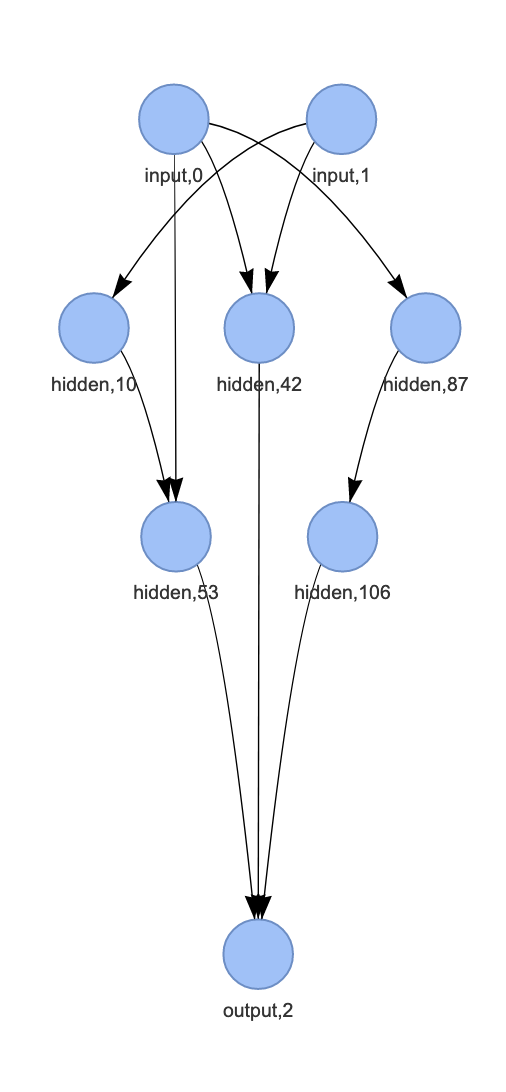
\includegraphics[width=0.8\textwidth]{xor_topology_example.png}
        \caption{An example topology of a genome that solves XOR problem without bias node }
        \label{fig:xor_bias}
    \end{figure}
    Second, the lack of dynamic threshold for specie distance calculation seems to make the problem harder to solve.
    This is less suprising, as the dynamic threshold is a mechanism that is supposed to help the algorithm in situations
    where the problem is hard to solve. What is suprising about this is that the difference in performance is so big for
    such a simple problem. This solution is also not very robust compared to the original one, achieving only 91.2\% success rate
    compared with 100\% of the original, and taking far more generations to find the solution.
\subsection{Cartpole}
    The results of cartpole trials are not very useful. The problem is solved in all 1000 trials, but the results suggest, that 
    this problem is too easy for the algorithm to be a good test of its capabilities. The average number of generations is 2.77, 
    meaning that the algorithm is able to solve the problem in less than 3 generations on average. To solve cartpole problem, the
    algorithm doesn't need to evolve any structure, as the starting topology is enough to solve the problem. The problem is therefore
    not inspected further.
\subsection{Acrobot}
    Solution to the acrobot problem is showing more promise than the cartpole, but ultimately also fails to provide a 
    good challenge to the algorithm. The problem is solved in all 1000 trials, and even though the average number of generations is up, it 
    is still only 4.45. The average number of nodes and connections in the solution is also very low, with 8.95 and 17.07 respectively. 
    Given that the minimal starting genome for this problem has 8 nodes and 15 connections, it is safe to say this problem can be 
    categorized as trivial.
\subsection{Walker}
    The case of bipedalwalker is a curious one. The model can reliably learn to walk to the end of the map (corresponding
    to this is fitness of about ~150-200). It cannot however finish the course with a cumulative fitness required by the
    environment. How is that possible? The environment in bipedalwalker has total fitness requirement of 300, divided
    into small chunks given to an agent by moving forward. However, environment also keeps track of the movement made
    by the agent, and reduces reward based on the 'energy-efficiency' of its movements. In this situation agent 
    gets terminated by the environment (has walked to the end of the map), but doesn't have enough fitness to be 
    qualified as a win. 
    This is problematic, as the fitness function used by the algorithm (and the gymnasium environment
    itself) is not suited well for teaching agents to walk efficiently. There is enough noise inbetween
    randomly generated maps, that the difference in fitness from a good run and a bad run is more reliant
    on the map itself than the agent's efficiency in performance.
     That is because once the agent learns to walk, the reward it gets from simply moving forward is higher than any influence
     of the energy-efficiency correction. This means that the agent is not incentivized to walk efficiently, and
     once it gets to the end of the map consistently, there is no clear way for it to improve its fitness (the 
     act of walking efficiently seems to need far more structure, which is hard to evolve when there is small 
     reward to be gained at this point.
      )
    are very long, with the fitness being reduced by the environment constituting a very small part of the total fitness missing.
\section{Future work}
    Proposed future work is divided into two categories: 
        \subsection{Improvements to the visualization} 
        To make the didactic part of the implementation more useful, it would be good to add a visualization of the
        learning process. Current version permits user to dump data from the learning process, which is used to
        generate graphs representing state of the select genomes in the network. This is a good start, but is not
        a very user-friendly way of interacting with the system. It would be better to have a live visualization.
        Currently in the codebase, there is also no code for plotting the specie perormance over time, which would
        help in understanding the speciation process.
        \subsection{Improvements to the performance}
        The current implmenentation focused on simplicity, and therefore is not very performant. And while performance
        is not a stated priority, it there are some ways to improve it without sacrificing much of the simplicity.
        The evaluation of the genomes is currently done in a single thread, which is a bottleneck for the whole process.
        It would be good to implement a multithreaded evaluation, which would speed up the process significantly.
\section{TODO \& Notes}
\begin{itemize}
    \item Opisać problem napotkany przy uzyciu negatywnego fitnessu, tak jak w https://www.cs.ucf.edu/~kstanley/neat.html , 
    sekcja "dobieranie problemów do algorytmu"?
    quote:

"Is there a way to use negative fitnesses in NEAT?
You may have noticed that if you try to use negative fitnesses, NEAT breaks down because of fitness sharing, which requires positive fitness values.
Real Carbonneau suggested the following solution to this problem: Compute fitness as you wish, with negative values if desired. Then, adjust all the fitnesses by replacing them with the distance between the actual fitness and the lowest fitness in the population. This will scale all the fitnesses above zero, keeping the relationships stable. "
\item cytowania; pomysły: rzeczy z orginalnego papera o TWEANN i metodach, strona autora https://www.cs.ucf.edu/~kstanley/neat.html, strona hyperNeata (do omówienia extensions)
\item neuroevolution vs gradient descent
\end{itemize}
\bibliography{references}
\end{document}